\subsection{H1-hESC cell line} \label{meth-encode-h1-subsect}
The same experiment was conducted for clustering DNA methylation profiles for the H1-hESC cell line. As promoter regions were considered 1000bp upstream and 1000bp downstream of the TSS, resulting in 2000bp in total. This resulted in 5,270 promoter regions for testing. The total number of clusters K was set to 5, and the methylation profiles were modelled using $5^{th}$ degree polynomials. 

Similarly to \emph{Fig. \ref{meth-k562-pic}}, figures \emph{\ref{methH1:first}} and \emph{\ref{methH1:second}} depict the five methylation profiles that are fitted to the promoter regions of the H1-hESC data, and the corresponding expression levels of the protein coding genes assigned to each cluster K, respectively.
\begin{figure}[ht!]
     \begin{center}
        \subfigure[]{
            \label{methH1:first}
            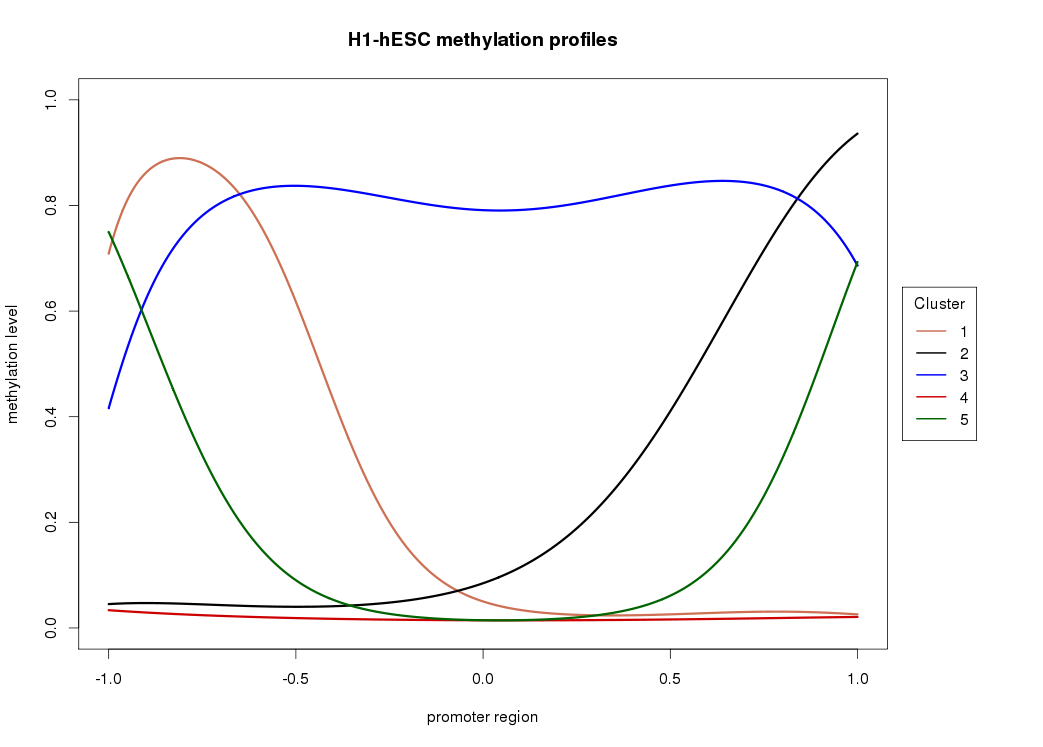
\includegraphics[width=0.45\textwidth]{images/h1MethProfClusters}
        }
        \subfigure[]{
           \label{methH1:second}
           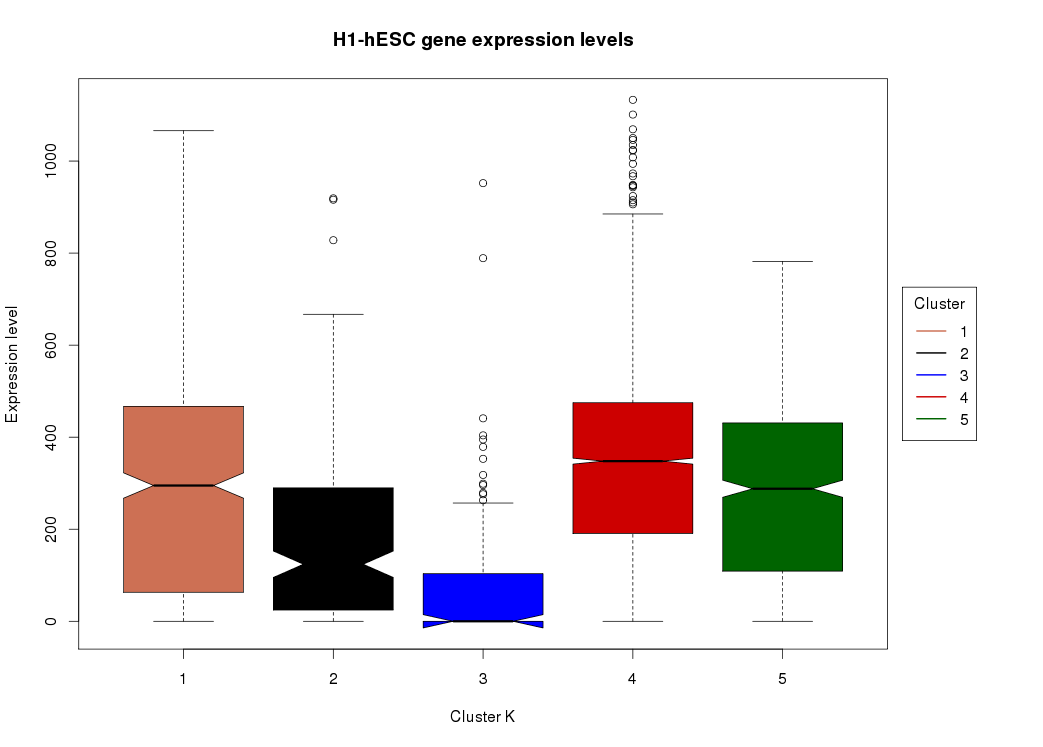
\includegraphics[width=0.495\textwidth]{images/h1MethProfBoxPlot}
        }
    \end{center}
    \caption{\emph{(a) Clustering DNA methylation profiles for the H1-hESC cell line with $5^{th}$ degree polynomial, each colour represents a different cluster. (b) Boxplot with the corresponding gene expression levels of the protein-coding genes assigned to each cluster K for the H1-hESC cell line. See the text for details.}}
   \label{meth-H1-pic}
\end{figure}